\documentclass{article}
\title{Entregable Representación Gráfica}
\author{Alejandro Zubiri}

\usepackage{amsmath, physics, amsfonts, amsthm, graphicx}

\graphicspath{ ../images/}

\begin{document}
\maketitle
\tableofcontents
\pagebreak
Queremos representar la siguiente función:
\begin{equation}
	\begin{split}
		f(x) = \frac{1}{x} + \ln |x|
	\end{split}
\end{equation}
\section{Dominio}
El dominio de la función es:
\begin{equation}
	\begin{split}
				\text{Dom }f = \mathbb{R}- \{ 0 \} 
	\end{split}
\end{equation}
\section{Asíntotas}
\subsection{Verticales}
El único punto conflictivo es en \(x=0\):
\begin{equation}
	\begin{split}
		\lim_{x \to 0} \frac{1}{x} + \ln |x| = 
		 \left\{\begin{matrix}
\lim_{x \to 0^{-}} \frac{1}{x}+ \ln |x|= -\infty \\
\lim_{x \to 0^{+}} \frac{1}{x} + \ln |x| = \infty 
\end{matrix}\right.
	\end{split}
\end{equation}
Por tanto, hay una asíntota vertical en \(x=0\).
\subsection{Horizontales}
\begin{equation}
	\begin{split}
		\lim_{x \to \infty} \frac{1}{x}+ \ln |x|&= \infty\\
		\lim_{x \to -\infty} \frac{1}{x}+ \ln |x| &= \lim_{x \to \infty} - \frac{1}{x} + \ln |x|
		=\infty  
	\end{split}
\end{equation}
\subsection{Oblicuas}
La pendiente de la recta oblicua en \(+\infty\) es:
\begin{equation}
	\begin{split}
		m = \lim_{x \to \infty} \frac{f(x)}{x}=
		\lim_{x \to \infty} \frac{1}{x^{2}} = \frac{\ln |x|}{x}=
	\end{split}
\end{equation}
La primera parte tiende a 0, y al tener una indeterminación de tipo \(\frac{\infty}{\infty}\),
aplicamos L'Hôpital:
\begin{equation}
	\begin{split}
		= \lim_{x \to \infty} \frac{1}{x}=0
	\end{split}
\end{equation}
Por tanto, no hay asíntota oblicua en \(+\infty\). Si miramos en \(-\infty\):
\begin{equation}
	\begin{split}
		m=\lim_{x \to -\infty} \frac{1}{x^{2}} + \frac{\ln |x|}{x}
		= \lim_{x \to \infty} \frac{1}{x^{2}}- \frac{\ln |x|}{x}
		= \lim_{x \to \infty} -\frac{1}{x}=0
	\end{split}
\end{equation}
De nuevo, podemos aplicar L'Hôpital para obtener un resultado similar, donde vemos que tampoco
hay asíntota oblicua en \(-\infty\).
\section{Monotonía y extremos relativos}
La derivada de la función es:
\begin{equation}
	\begin{split}
		f'(x)=\dv{f}{x}= \frac{x-1}{x^{2}}
	\end{split}
\end{equation}
Podemos igualar a \(0\) para encontrar los extremos relativos:
\begin{equation}
	\begin{split}
		f'(x)=0 \implies x-1=0 \implies x=1
	\end{split}
\end{equation}
Si evaluamos la derivada en puntos cercanos al extremo, vemos que por la izquierda es negativa,
y que por la derecha es positiva, lo que indica que \(x=1\) es un mínimo relativo.\\
Además, la función es decreciente \(\forall x \in (-\infty, 1)\) y creciente
\(\forall x \in (1, \infty)\).
\section{Curvatura}
La segunda derivada de la función es:
\begin{equation}
	\begin{split}
		f''(x) = \dv[2]{f}{x}= \frac{2-x}{x^{3}}
	\end{split}
\end{equation}
Para obtener los puntos donde la curvatura cambia, igualamos la segunda derivada a \(0\),
obteniendo:
\begin{equation}
	\begin{split}
		f''(x)=0 \implies 2-x = 0 \implies x = 2
	\end{split}
\end{equation}
De nuevo, evaluando a la izquierda la segunda derivada es positiva, y a la derecha es negativa,
lo que indica que la función es cóncava hacia abajo \(\forall x \in (-\infty, 2)\) y cóncava
hacia arriba \(\forall x \in (2,+\infty)\).
\section{Boceto y representación}
Evaluando en algunos puntos podemos realizar el siguiente boceto de la función:
\begin{table}[h]
	\begin{tabular}{lllll}
	x & f(x)\\
	1 & 1\\
	-1 & -1\\
	-2 & 0.19 \\
	-3 & 0.76
	\end{tabular}
\end{table}
\begin{figure}[h]
	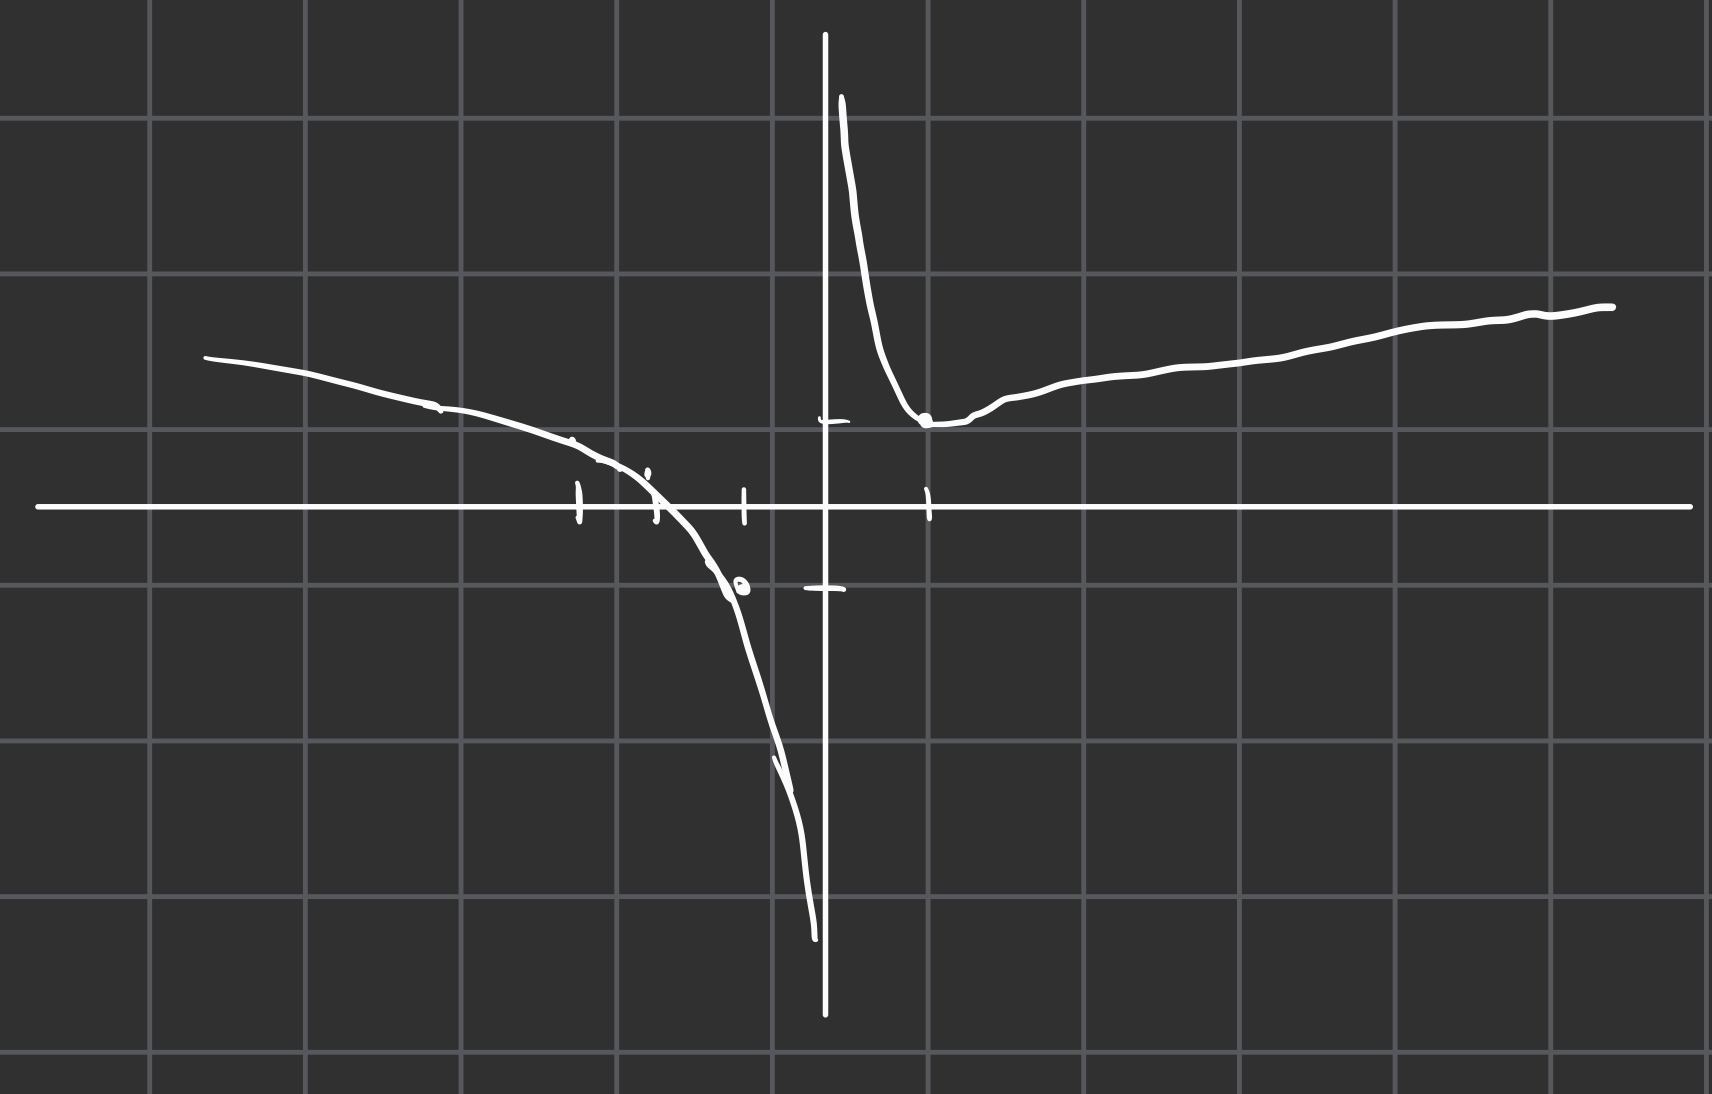
\includegraphics[scale=0.25]{../images/20241228_134027000_iOS.jpg}
\end{figure}
\section{Imagen}
Una vez hemos analizado la función, podemos afirmar que la imagen de la función es:
\begin{equation}
	\begin{split}
		\text{Im }f= \mathbb{R}
	\end{split}
\end{equation}
\end{document}
